\subsection{Thermal-Hydraulics Analysis}
Preliminary checks were conducted on coolant properties.

Density, viscosity, and thermal conductivity were validated at the coolant inlet temperature.

The heat transfer coefficient between the coolant and cladding was computed using Nusselt number correlations.

Figure~\ref{fig:thermal_hydraulics} shows the axial power profile. the computed heat transfer coefficient in cold geometry was $\alpha_{coolant} = 139.98 \frac{kW}{m^2 K}$.

\begin{figure}[H]
    \centering
    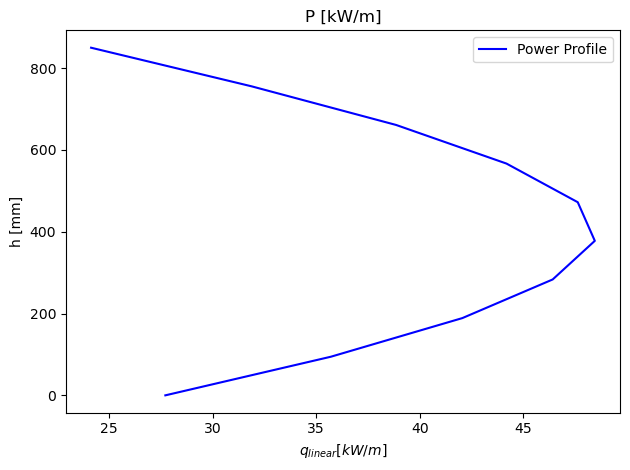
\includegraphics[width=0.8\textwidth]{power_profile.png}
    \caption{Thermal-hydraulics analysis results.}
    \label{fig:thermal_hydraulics}
    \end{figure}